\chapter{WinEdt v9 and Below}
\section{Adding a Custom Button}

\begin{numberedlist}
	\item Open: \textcode{Options$\rightarrow{}$Preferences$\rightarrow{}$Advanced}
	
	\item Edit the \textcode{WinEdt.btn} file as shown in \figurename~\ref{fig:addcustombutton}.
	
	\item Add a line to the end of the file similar to:
	\begin{plainlist}
		\item \textcode{204 \%B\tbs{}Bitmaps\tbs{}Buttons\tbs{}Command Prompt.bmp}
		\item \textcode{205 \%B\tbs{}Bitmaps\tbs{}Buttons\tbs{}Recycle.bmp}
		\item \textcode{206 \%B\tbs{}Bitmaps\tbs{}Buttons\tbs{}Recycle.bmp}
		\item \textcode{207 \%B\tbs{}Bitmaps\tbs{}Buttons\tbs{}image.bmp}
	\end{plainlist}
\end{numberedlist}
The number in that line will be the button number is the toolbar setup.
Use a BMP from one previously defined.
\begin{figure}
	\centering
	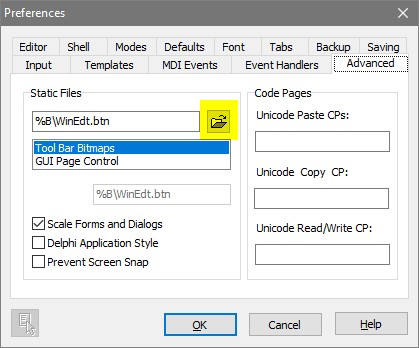
\includegraphics[width=3in]{addcustombutton}
	\caption[Edit the \textcode{WinEdt.btn}]{Edit the \textcode{WinEdt.btn}.}
	\label{fig:addcustombutton}
\end{figure}



\section{Add a New Command}
Enter the menu setup as shown in \figurename~\ref{fig:entermenusetup}.
\begin{figure}
	\centering
	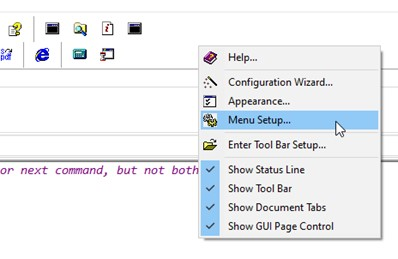
\includegraphics[width=3in]{entermenusetup}
	\caption[Enter menu setup]{Enter menu setup.}
	\label{fig:entermenusetup}
\end{figure}

Double click an entry (as shown in \figurename~\ref{fig:doubleclickmenuitemtoopen} to open it for editing.
\begin{figure}
	\centering
	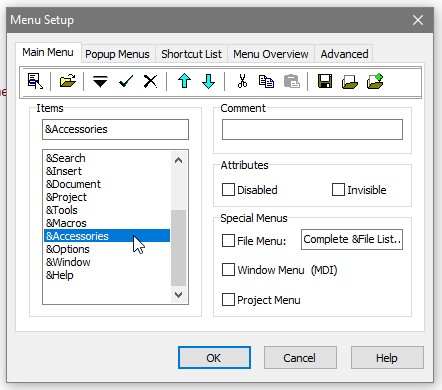
\includegraphics[width=3in]{doubleclickmenuitemtoopen}
	\caption[Double click the menu item to open the editor for it]{Double click the menu item to open the editor for it.}
	\label{fig:doubleclickmenuitemtoopen}
\end{figure}

Setup all the highlighted sections in \figurename~\ref{fig:commandsetup}.  The commands to use are below.
\begin{plainlist}
	\item Make Document
	\begin{plainlist}
		\item Macro:    \textcode{Run('run\_make\_document.bat "\%N"','',0,0,'Make Document',1,1);}
		\item Start in: \textcode{\%P}
	\end{plainlist}
		\item Clean Temp Files
	\begin{plainlist}
		\item Macro:    \textcode{Run('clean\_temp\_files.bat','',0,0,'Clean Up',1,1);}
		\item Start in: \textcode{\%P}
	\end{plainlist}
		\item Clean All Output
	\begin{plainlist}
		\item Macro:    \textcode{Run('clean\_all\_output.bat','',0,0,'Clean Up',1,1);}
		\item Start in: \textcode{\%P}
	\end{plainlist}
		\item Convert All Images
	\begin{plainlist}
		\item Macro:    \textcode{Run('convert\_all\_images.bat','',0,0,'Make Images',1,1);}
		\item Start in: \textcode{\%P\tbs{}Figures\tbs{}Image Sources\tbs{}}
	\end{plainlist}
\end{plainlist}

\begin{figure}
    \centering
    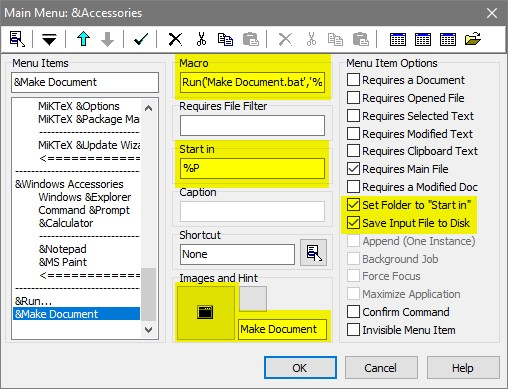
\includegraphics[width=3in]{commandsetup}
    \caption[Ensure all the highlighted sections are set correctly]{Ensure all the highlighted sections are set correctly.}
    \label{fig:commandsetup}
\end{figure} 